\documentclass[11pt, letterpaper]{article}
\usepackage[margin=1in]{geometry}
\usepackage{tikz}
\usepackage[american, siunitx]{circuitikz}
\usepackage{amsmath}
\usepackage{ulem} % 用于下划线

% 取消默认的段落缩进，增加段落间距，以匹配原文档风格
\setlength{\parindent}{0pt}
\setlength{\parskip}{1em}

\begin{document}

\textit{Please show your work}

\textbf{Problem 1: Analysis of inverting and non-inverting amplifier structures}

\begin{center}
    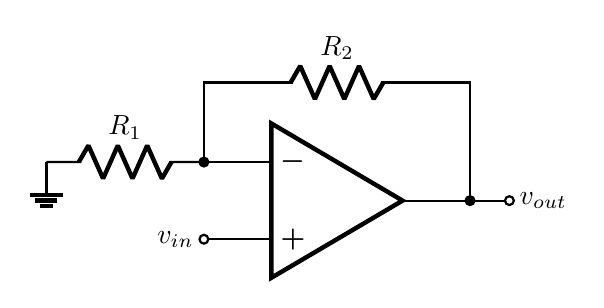
\begin{tikzpicture}[american, thick]
        % 运算放大器
        \node[op amp] (OA) at (0,0) {};
        
        % 同相输入端 (+) 接 vin
        \draw (OA.+) -- ++(-0.5,0) node[ocirc]{} node[left]{$v_{in}$};
        
        % 反相输入端 (-) 节点
        \coordinate (in_node) at ($(OA.-) + (-0.5,0)$);
        \draw (OA.-) -- (in_node);
        \node[circ] at (in_node) {}; 
        
        % 接地电阻 R1
        \draw ($(in_node) + (-2,0)$) node[ground]{} to[R, l=$R_1$] (in_node);
        
        % 输出端节点与 vout
        \draw (OA.out) to[short, -*] ++(0.5,0) coordinate (out_node);
        \draw (out_node) to[short, -o] ++(0.5,0) node[right]{$v_{out}$};
        
        % 反馈电阻 R2 回路 (强制水平对齐)
        \coordinate (fb_level) at (0, 1.5); 
        \coordinate (fb_lt) at (in_node |- fb_level);
        \coordinate (fb_rt) at (out_node |- fb_level);
        \draw (in_node) -- (fb_lt) to[R, l=$R_2$] (fb_rt) -- (out_node);
    \end{tikzpicture}
    
    \vspace{0.5em}
    \textbf{Figure 1a. Non-inverting amplifier}
\end{center}

\vspace{1em}

\begin{center}
    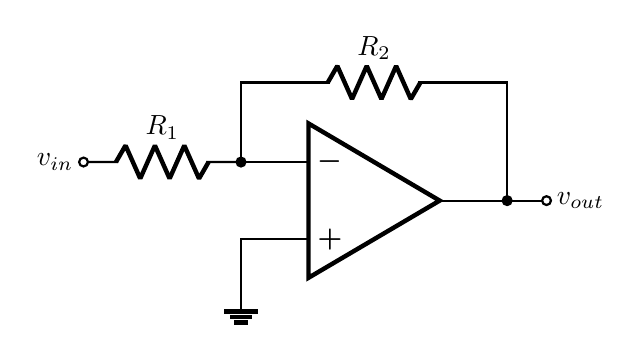
\begin{tikzpicture}[american, thick]
        % 运算放大器
        \node[op amp] (OA) at (0,0) {};
        
        % 同相输入端 (+) 接地
        \draw (OA.+) -- ++(-0.5,0) coordinate (pos_node) -- ++(0,-0.5) node[ground]{};
        
        % 反相输入端 (-) 节点
        \coordinate (in_node) at ($(OA.-) + (-0.5,0)$);
        \draw (OA.-) -- (in_node);
        \node[circ] at (in_node) {}; 
        
        % 输入电阻 R1 和 vin
        \draw ($(in_node) + (-2,0)$) node[ocirc]{} node[left]{$v_{in}$} to[R, l=$R_1$] (in_node);
        
        % 输出端节点与 vout
        \draw (OA.out) to[short, -*] ++(0.5,0) coordinate (out_node);
        \draw (out_node) to[short, -o] ++(0.5,0) node[right]{$v_{out}$};
        
        % 反馈电阻 R2 回路 (强制水平对齐)
        \coordinate (fb_level) at (0, 1.5); 
        \coordinate (fb_lt) at (in_node |- fb_level);
        \coordinate (fb_rt) at (out_node |- fb_level);
        \draw (in_node) -- (fb_lt) to[R, l=$R_2$] (fb_rt) -- (out_node);
    \end{tikzpicture}
    
    \vspace{0.5em}
    \textbf{Figure 1b. Inverting amplifier}
\end{center}

\vspace{1em}

Most closed-loop amplifiers involving opamps are some variation on either the inverting or non-inverting amplifier. For this reason, it is important to be familiar with these structures and their characteristics.

For the following, $R_1 = 1k\Omega$ and $R_2 = 9k\Omega$

For the opamp(s), DC open-loop gain $A_0 = 10^6 V/V$, open-loop input resistance $R_{in} \rightarrow \infty$, and open-loop output resistance $R_{out} = 1k\Omega$

\underline{\textit{DC Analysis}}

\textbf{a)} Determine the \textit{closed-loop} gain, input resistance, and output resistance for each (inverting and non-inverting) amplifier.

\textbf{b)} If the opamp has a voltage offset $v_{os} = 1mV$ and input bias current $I_b = 1nA$, determine the total output offset voltage for each amplifier. It will be helpful to use superposition for this.

\vspace{1.5em}

\textbf{Problem 2: Sensor amplification}

\begin{center}
    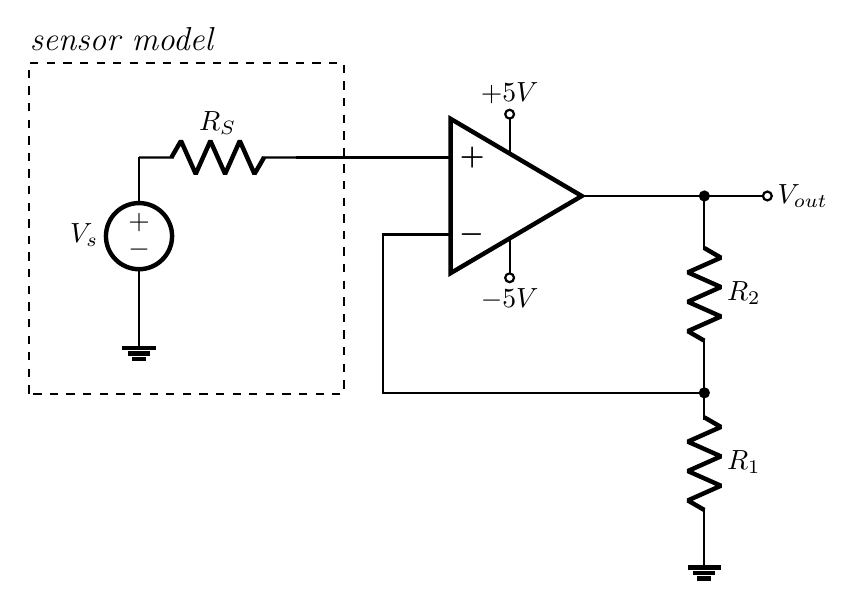
\begin{tikzpicture}[american, thick]
        % 运算放大器 (Op-amp)
        \node[op amp, noinv input up] (OA) at (0,0) {};
        
        % 电源引脚
        \draw (OA.up) -- ++(0,0.5) node[ocirc]{} node[above]{$+5V$};
        \draw (OA.down) -- ++(0,-0.5) node[ocirc]{} node[below]{$-5V$};
        
        % 输出端与分压电阻网络 (R2 和 R1)
        \draw (OA.out) to[short, -*] ++(1.2,0) coordinate (out_junct);
        \draw (out_junct) to[short, -o] ++(0.8,0) node[right]{$V_{out}$};
        
        % R2 向下连接
        \draw (out_junct) to[R, l=$R_2$] ++(0,-2.5) coordinate (fb_node);
        
        % R1 向下连接至地
        \draw (fb_node) to[R, l=$R_1$] ++(0,-1.8) node[ground]{};
        \node[circ] at (fb_node) {};
        
        % 反馈回路 (从反相输入端连接至分压节点)
        \draw (OA.-) -- ++(-0.5,0) |- (fb_node);
        
        % 传感器模型 (Sensor model)
        \coordinate (rs_right) at ($(OA.+) + (-1.6,0)$);
        \draw (OA.+) -- (rs_right);
        
        % Rs 向左连接
        \coordinate (vs_top) at ($(rs_right) + (-2,0)$);
        \draw (rs_right) to[R, l_=$R_S$] (vs_top);
        
        % Vs 向下连接至地
        \coordinate (vs_bot) at ($(vs_top) + (0,-2)$);
        \draw (vs_top) to[V, l_=$V_s$] (vs_bot) node[ground]{};
        
        % 绘制虚线框和文字
        \coordinate (box_rt) at ($(OA.+) + (-1.0, 0)$);
        \coordinate (box_lt) at ($(vs_top) + (-1.4, 0)$);
        \coordinate (box_top) at ($(vs_top) + (0, 1.2)$);
        \coordinate (box_bot) at ($(vs_bot) + (0, -1.0)$);
        
        \draw[thick, dashed] (box_lt |- box_bot) rectangle (box_rt |- box_top);
        
        % 文本：紧贴虚线框左上角
        \node[anchor=south west, inner sep=0, yshift=4pt] at (box_lt |- box_top) {\large \textit{sensor model}};
    \end{tikzpicture}
\end{center}

The non-inverting amplifier structure has the advantage of high input impedance, making it suitable for interfacing with sensors with high output resistance.

Opamps have limits in terms of both output voltage and current that need to be considered when designing amplifier circuits.

For the sensor, $V_{S,DC} = 0V$ ($R_S$ is included for conceptual purposes only - it won't affect any of your calculations).

For the opamp, $A_0 = 10^6 V/V$, $f_t = 10MHz$, open-loop input resistance $R_{in} \rightarrow \infty$, and open-loop output resistance $R_{out} = 0\Omega$

\underline{\textit{Design/Simulation}}

\textbf{a)} Assuming an input signal range of $\pm 100mV$, design the amplifier (i.e. determine the gain) that maximizes the gain while ensuring the output voltage never exceeds 80\% of the supply rails of $\pm 5V$.

Assuming the opamp has a maximum output current of $10mA$, determine minimum values for $R_1$ and $R_2$ to ensure the output current never exceeds 80\% of the $10mA$ limit.

\textbf{b)} Derive an expression for the closed-loop gain of the amplifier as a function of frequency. Plot the gain and phase of the amplifier using Python. Calculate the frequency at which the amplifier closed-loop gain becomes 1\% lower than the ideal value calculated in \textit{Part a}.

\textbf{c)} Verify your design in LTspice using the \textit{UniversalOpamp2} component. Show that your design meets the requirements by running an AC simulation with the DC value of $V_S$ set to $100mV$. Include a schematic showing the resistor values and DC node voltages along with your AC simulation results.

\textbf{Bonus (1 point):} Propose a design that achieves the same gain with at least 2x the bandwidth using the \underline{same opamp specs}. Provide a schematic and AC simulation results that show your design achieves this.

\end{document}